\documentclass[e4_tp1_main.tex]{subfiles}
\begin{document}

\section{Funcionamiento real de una fuente DC/DC}

Combinando el circuito de disparo con la fuente diseñada en la sección previa, el circuito resulta:


\todo[inline]{dibujo del circuito en latex}

\subsection*{a) Curvas Simuladas}

Se toman por un lado las curvas correspondientes a la conmutación del transistor.

\begin{figure}[H]
\centering
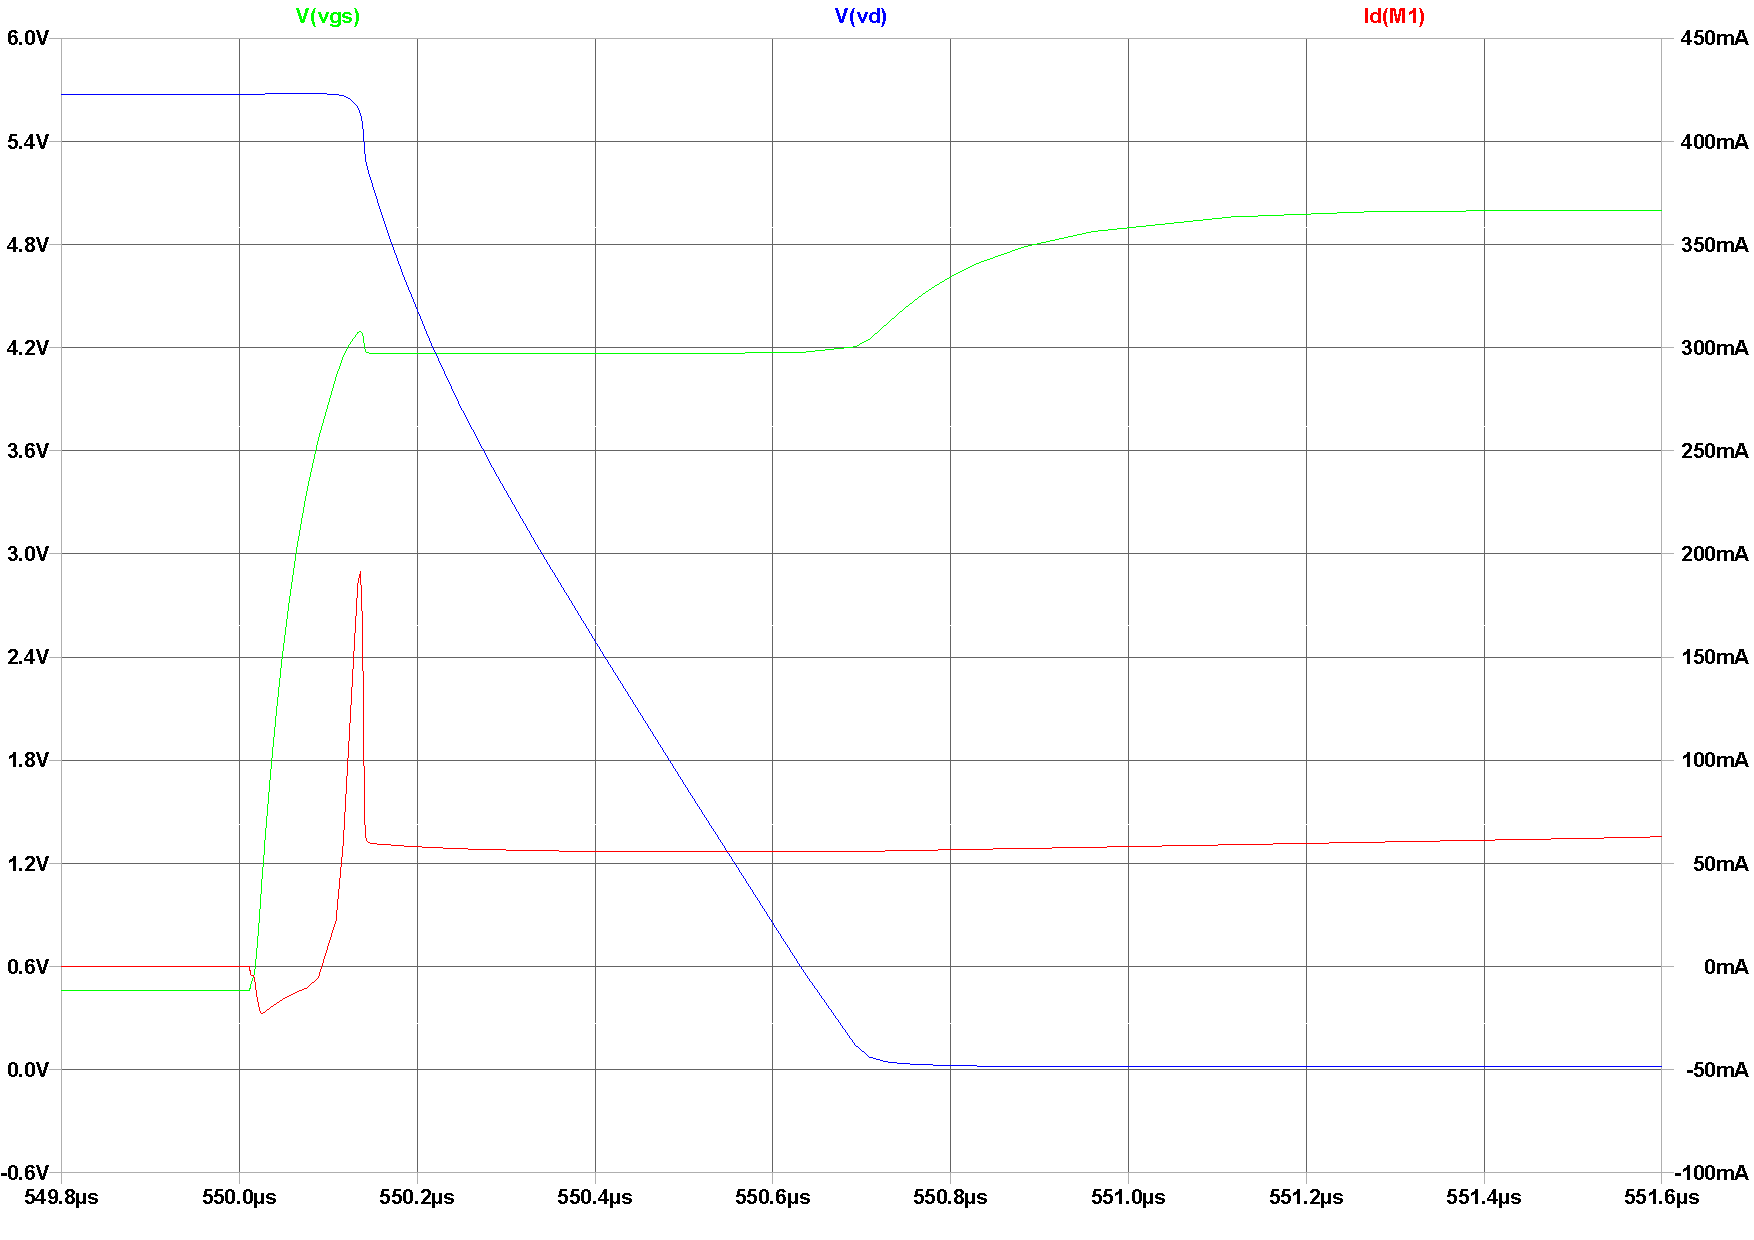
\includegraphics[width=0.7\linewidth]{Imagenes/Punto3/Encendido.pdf}
\end{figure}

De donde se tabulan los tiempos de encendido:

\[
t_d(ON) = 100nS \hspace{2cm} t_{ri} = 40nS \hspace{2cm} t_{fv} = 520nS
\]

\begin{figure}[H]
\centering
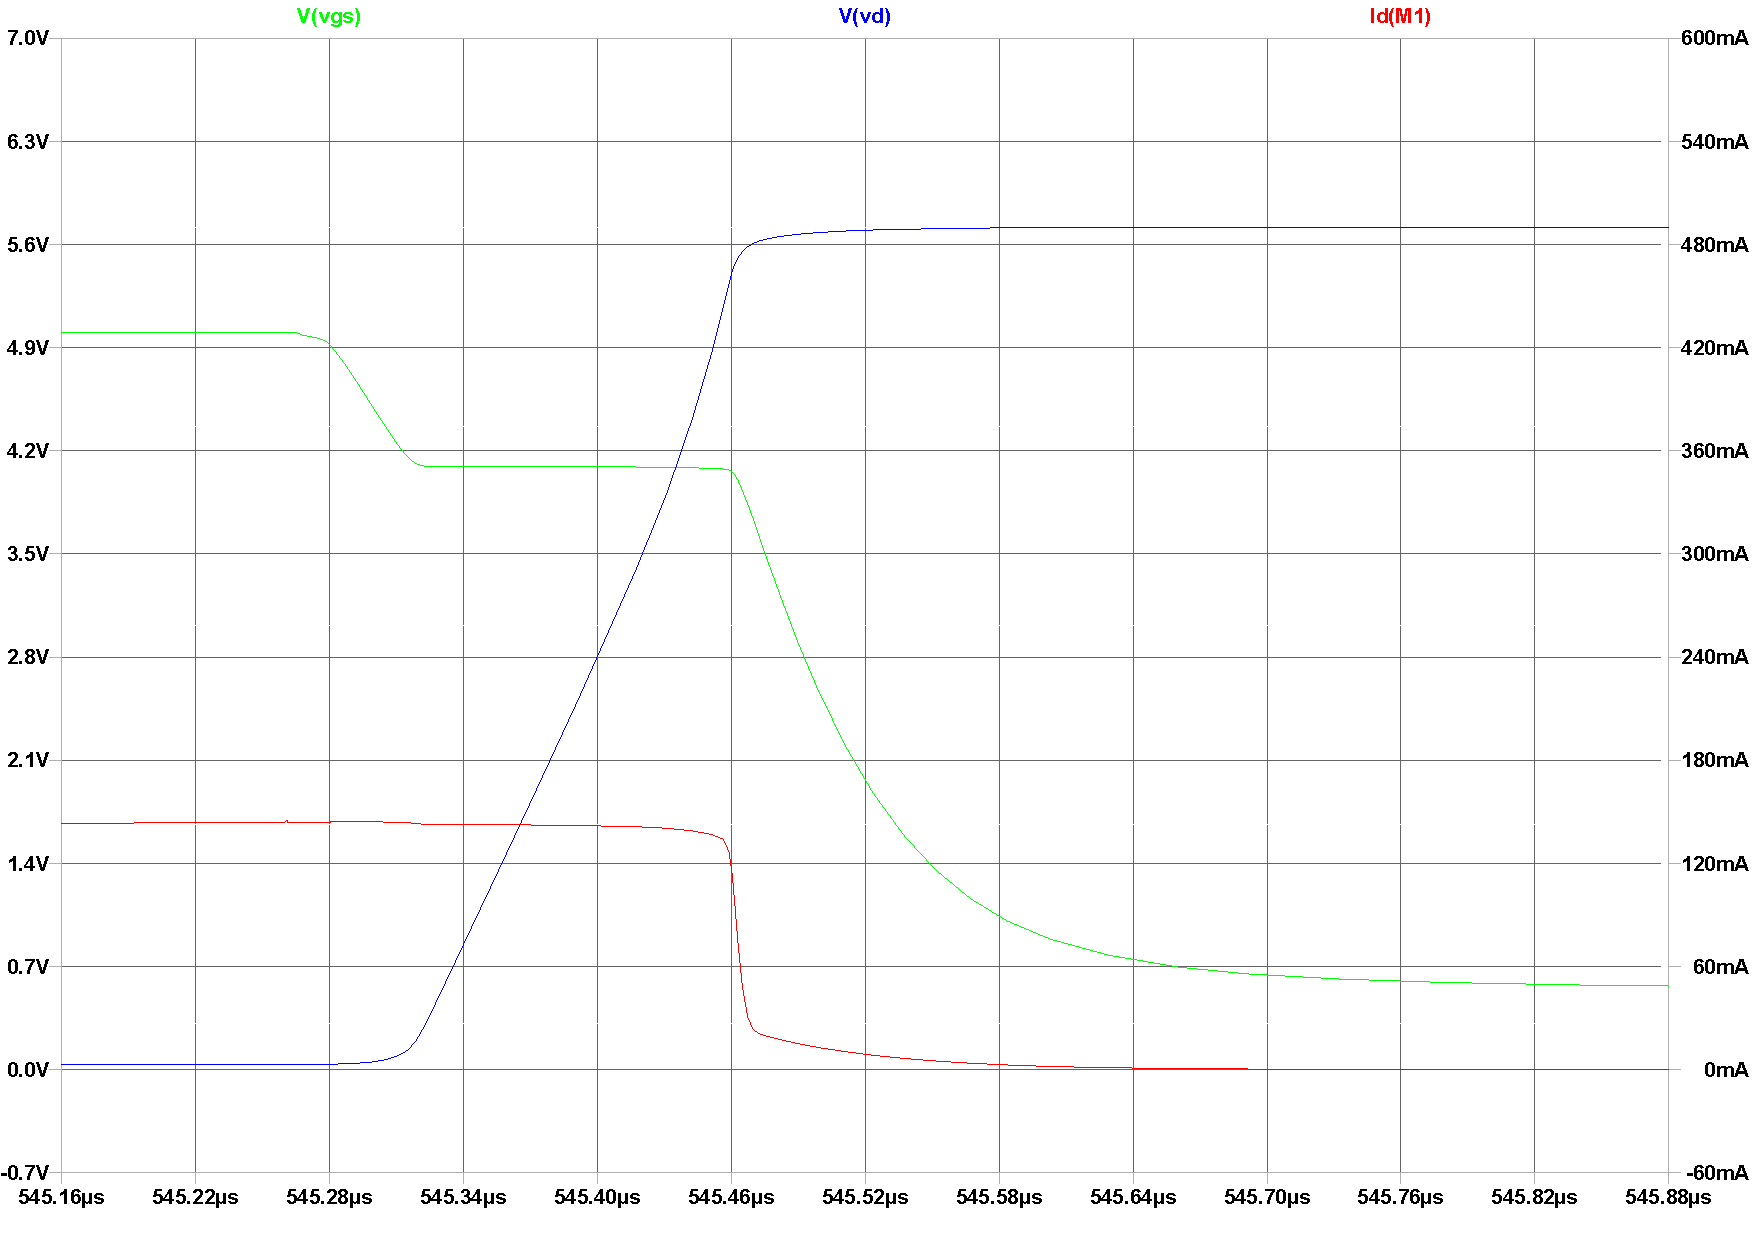
\includegraphics[width=0.7\linewidth]{Imagenes/Punto3/Apagado.pdf}
\end{figure}

De donde se tabulan los tiempos de apagado:

\[
t_d(OFF) = 60nS \hspace{2cm} t_{rv} = 120nS \hspace{2cm} t_{fi} = 20nS 
\]

Por otro lado, se toman las curvas de las tensiones y corrientes de los diferentes elementos:

\begin{figure}[H]
\centering
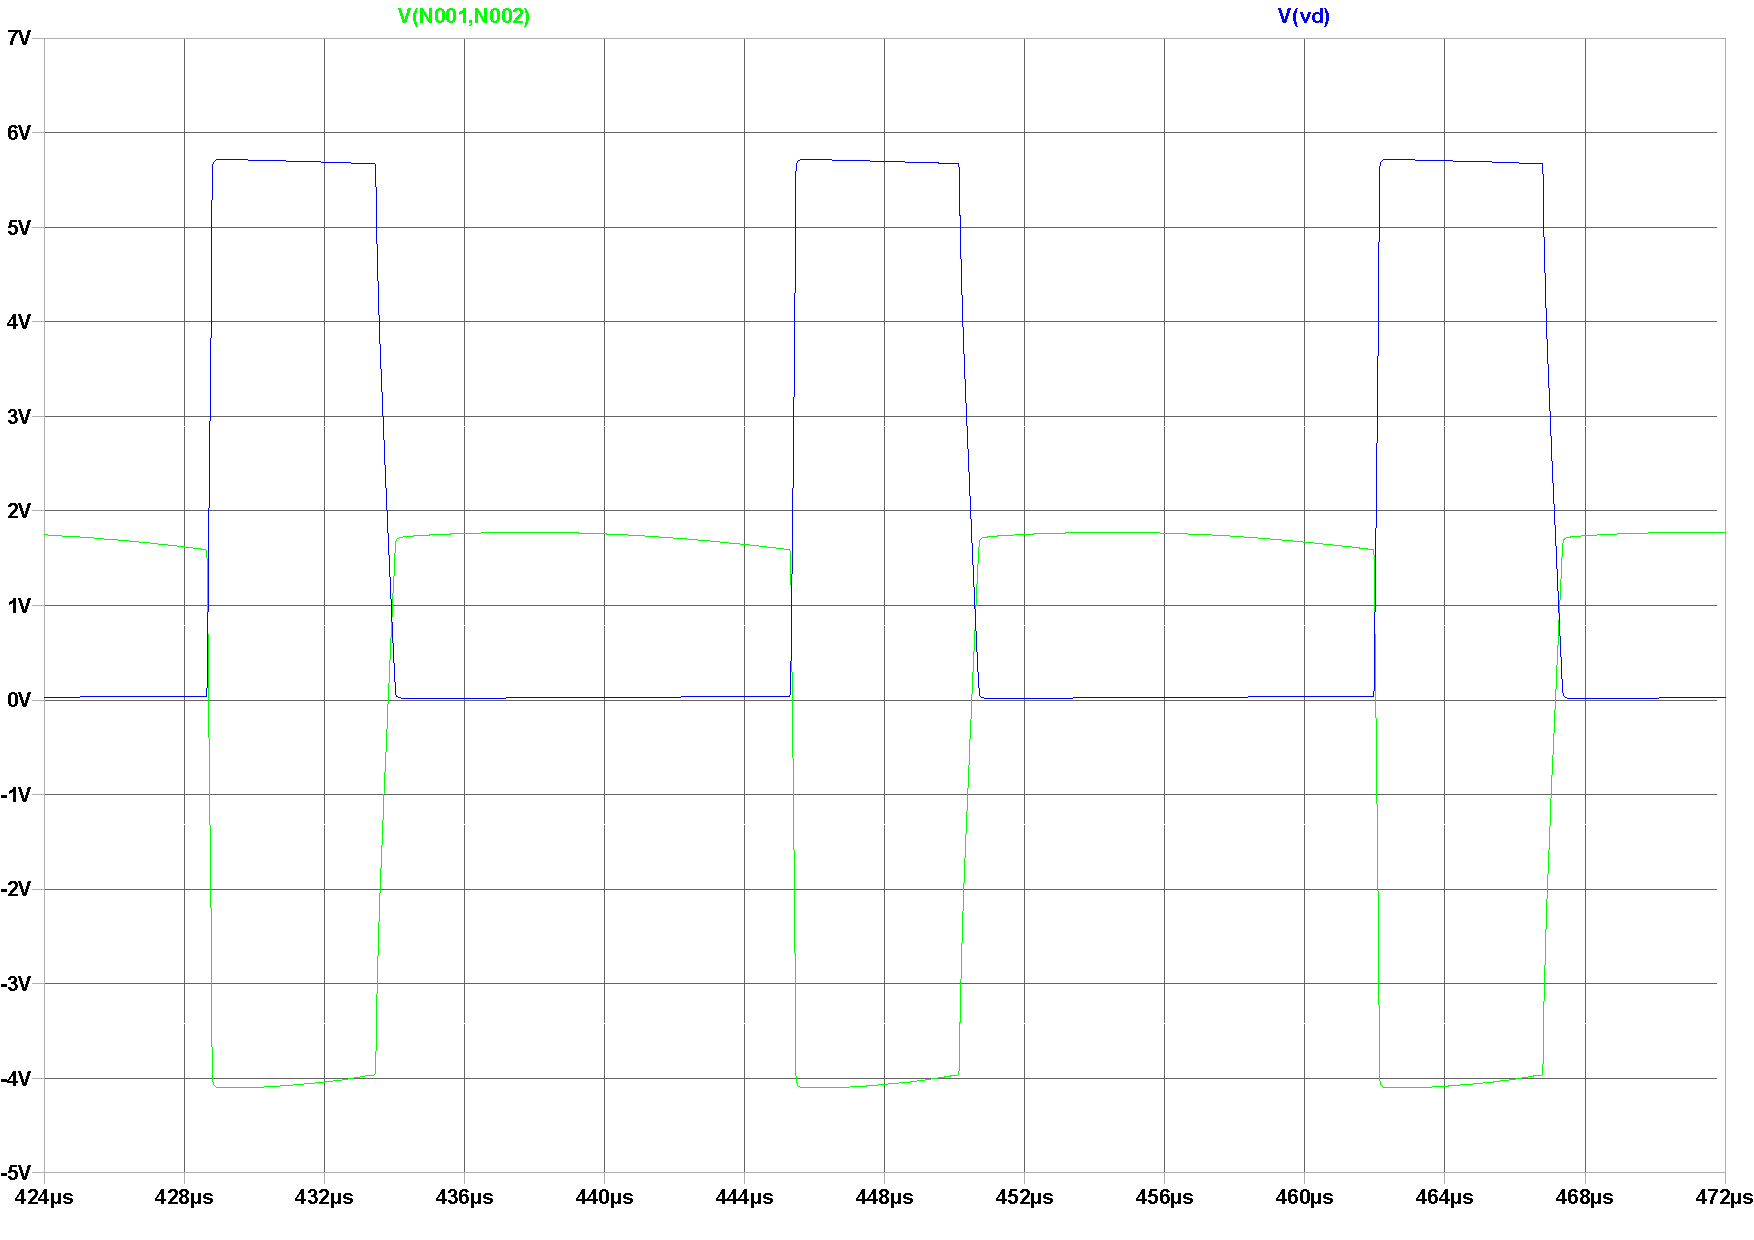
\includegraphics[width=0.7\linewidth]{Imagenes/Punto3/Sw-VL.pdf}
\caption{Simulación Sw(azul) y VL(verde)}
\end{figure}

\begin{figure}[H]
\centering
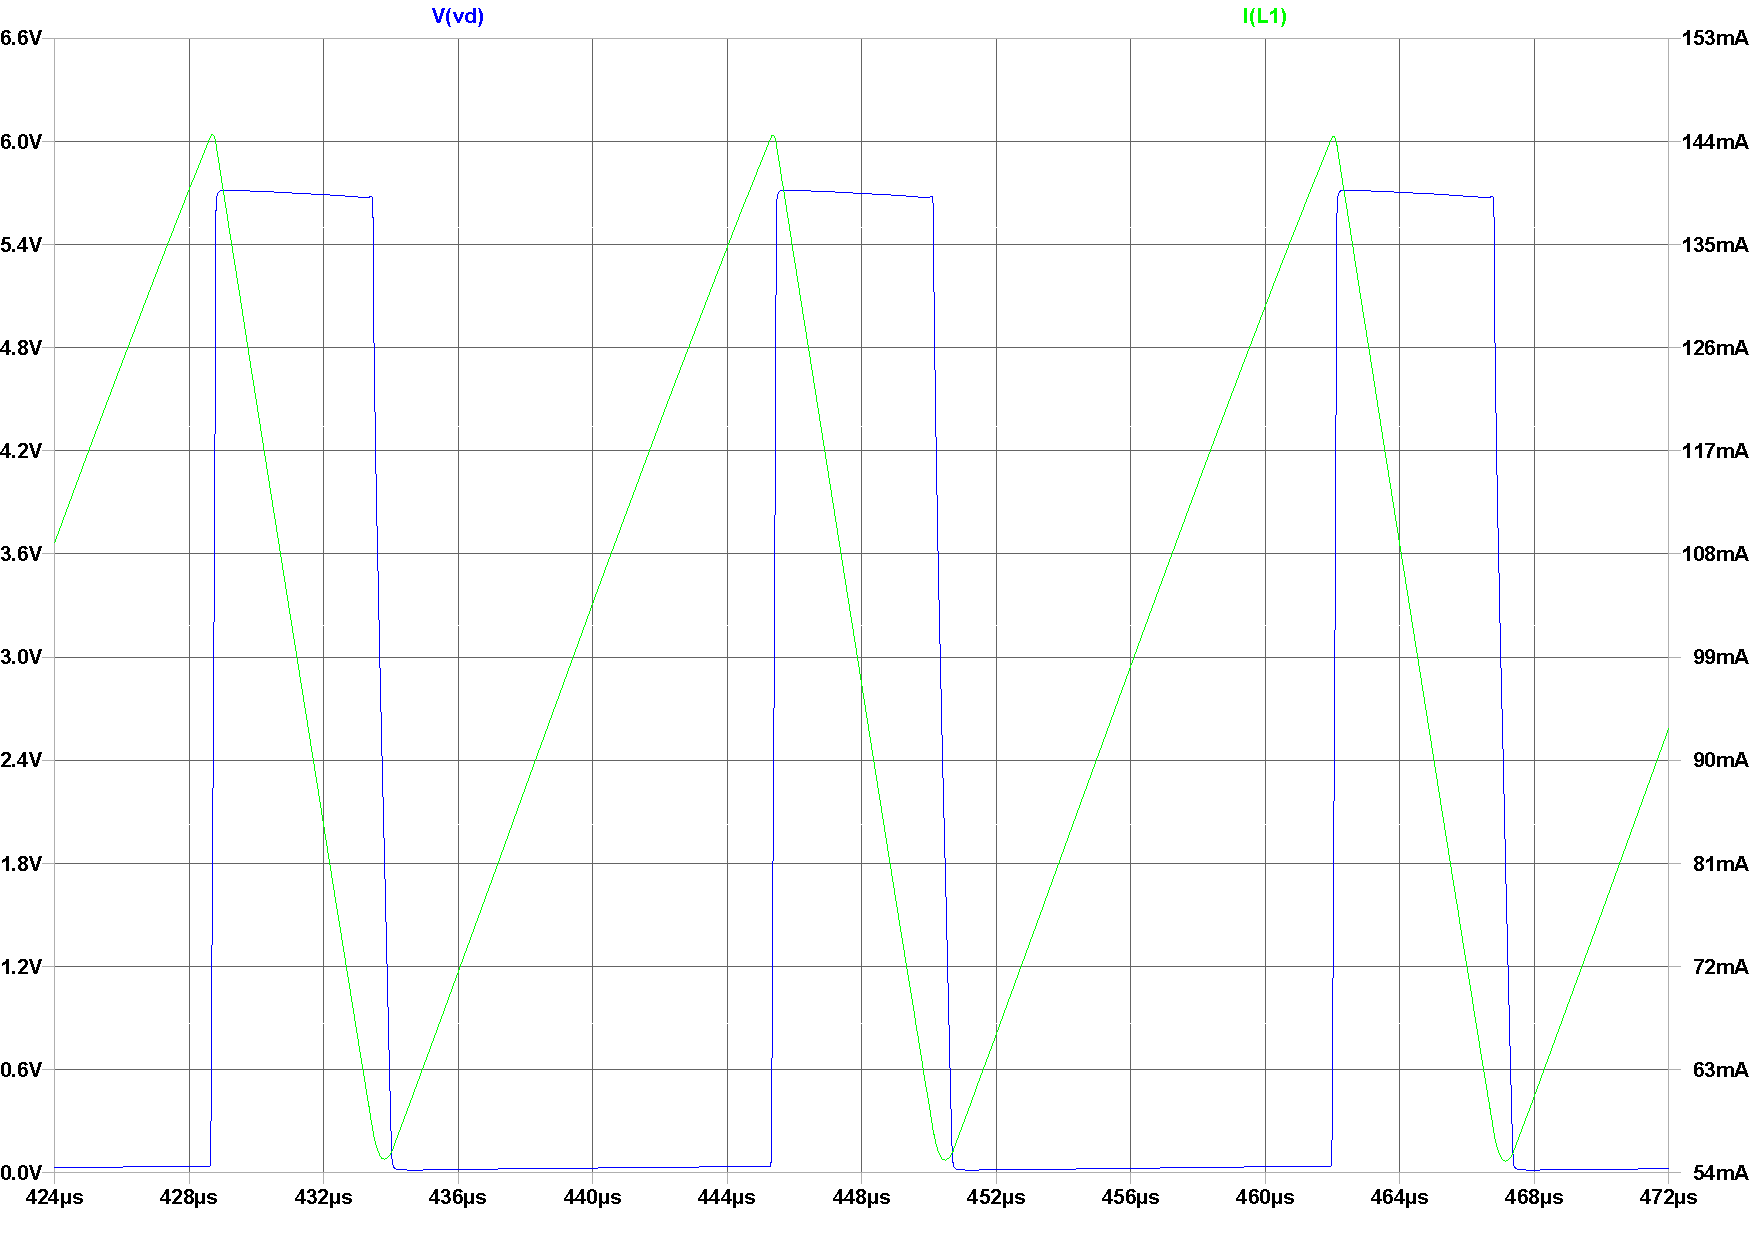
\includegraphics[width=0.7\linewidth]{Imagenes/Punto3/Sw-IL.pdf}
\caption{Simulación Sw(azul) y IL(verde)}
\end{figure}

\begin{figure}[H]
\centering
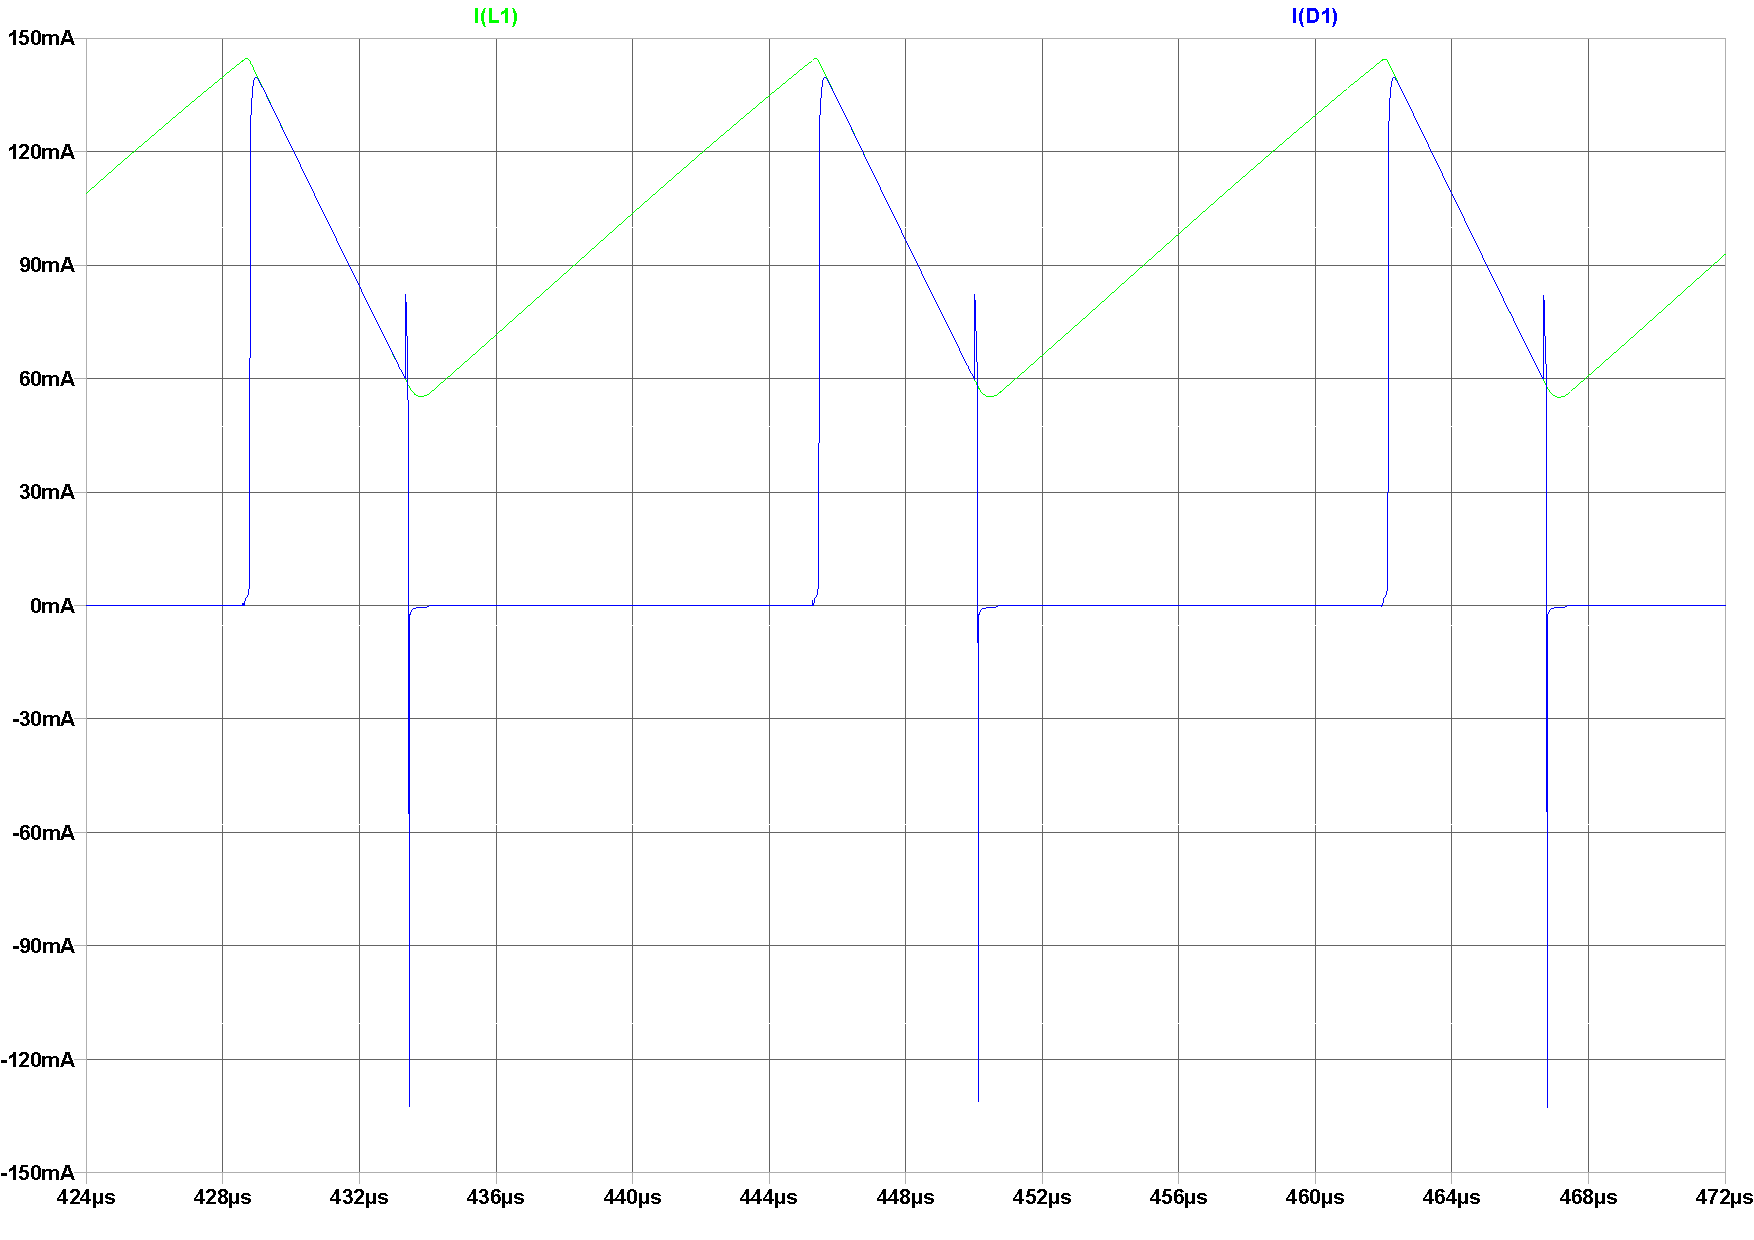
\includegraphics[width=0.7\linewidth]{Imagenes/Punto3/ID-IL.pdf}
\caption{Simulación ID(azul) y IL(verde)}
\end{figure}

\begin{figure}[H]
\centering
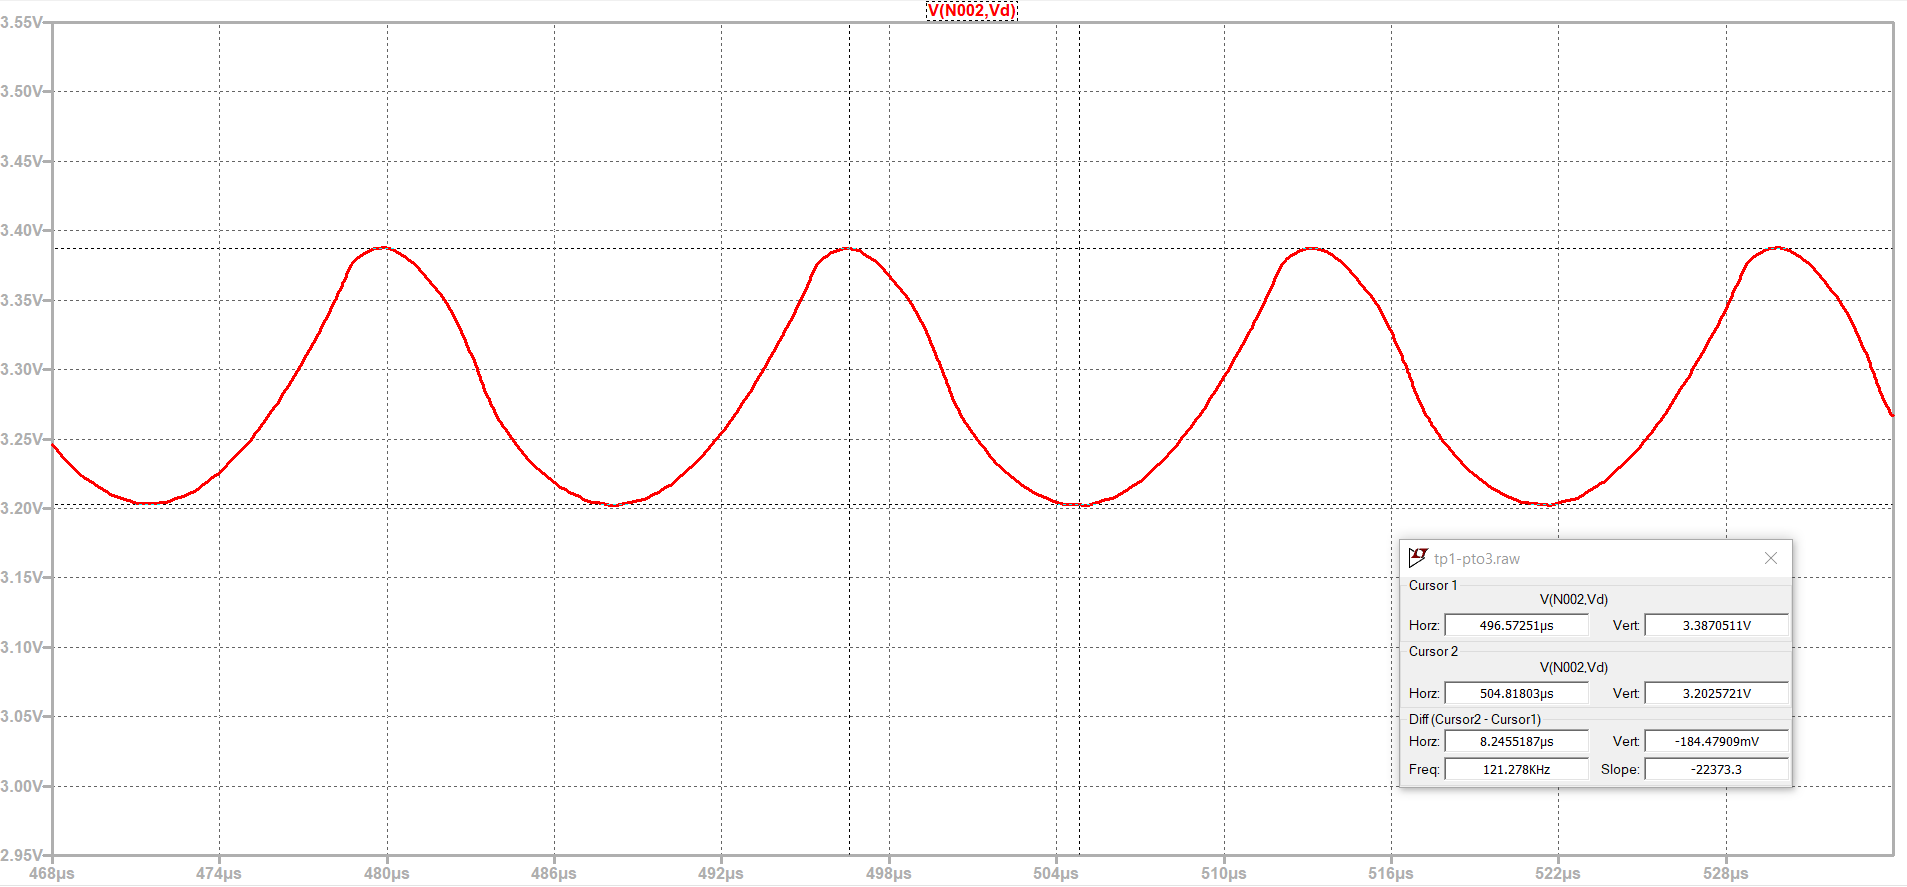
\includegraphics[width=0.9\linewidth]{Imagenes/Punto3/Vo.png}
\caption{Simulación salida $V_o$}
\end{figure}

\subsection*{b) Comparaciones y observaciones}



\newpage
\end{document}